%% csrlf.tex
%% 2014/03/24
%% by Hermann Yang

%import template
\documentclass[runningheads]{llncs}
\usepackage{amsmath, amssymb}
\usepackage{ruler}
\usepackage{color}

%\sloppy

% Custom packages
\usepackage{multirow}
\usepackage{paralist}

%% CITATION PACKAGES
\usepackage{cite}

%% GRAPHICS RELATED PACKAGES
\usepackage{graphicx}

%% ALIGNMENT PACKAGES
\usepackage{array}

%% SUBFIGURE PACKAGES
\usepackage[tight,footnotesize]{subfigure}

% PDF, URL AND HYPERLINK PACKAGES
\usepackage{url}

% FIX FOR SPANNING
\usepackage{stfloats}

% description list
\newcounter{desccount}
\newcommand{\desclabel}[1]{%
  \refstepcounter{desccount}\label{#1}
}

% correct bad hyphenation here
\hyphenation{op-tical net-works semi-conduc-tor}

\newcommand{\sys}{SRLF}

\newcommand{\csr}{CSR}

\newcommand{\lfea} {local feature-based algorithm}

\newcommand{\sregion} {salient region}

\makeatletter
\newcommand*{\rom}[1]{\expandafter\@slowromancap\romannumeral #1@}
\makeatother

\usepackage{times}
\usepackage[small,it]{caption}
\DeclareCaptionType{copyrightbox}

%\setlength{\abovecaptionskip}{-1pt}
%\setlength{\belowcaptionskip}{-1pt}
%\setlength{\textfloatsep}{2pt}
%\setlength{\floatsep}{2pt}
%\setlength{\intextsep}{4pt}

% save space for item size
\newcommand{\squishlist}{
 \begin{list}{$\bullet$}
  { \setlength{\itemsep}{0pt}
     \setlength{\parsep}{0pt}
     \setlength{\topsep}{1pt}
     \setlength{\partopsep}{0pt}
     \setlength{\leftmargin}{1.5em}
     \setlength{\labelwidth}{1em}
     \setlength{\labelsep}{0.5em} } }

\newcommand{\squishend}{
  \end{list}  }

%% DOCUMENT
\begin{document}

\pagestyle{headings}
\mainmatter

\def\ACCV14SubNumber{***}  % Insert your submission number here

%% TITLE
\title{\LARGE{{\sys}: Salient Region based Local Feature Extraction Algorithm}}


\titlerunning{ACCV-14 submission ID \ACCV14SubNumber}
\authorrunning{ACCV-14 submission ID \ACCV14SubNumber}

\author{Anonymous ACCV 2014 submission}
\institute{Paper ID \ACCV14SubNumber}


\maketitle
%% DOCUMENT BODY

\begin{abstract}
\setlength\parskip{9pt}

Local feature extraction algorithms have been widely used in different image or video retrieval systems. To guarantee the retrieval accuracy, they generally involve complex transformations and extract hundreds of high-dimension feature vectors to represent an image or a video frame. Although such a design can guarantee retrieval accuracy, it leads to a great pressure on real-time processing and large-scale storage with sharply increasing multimedia data.In an image or a video frame, there exist some human visual attention regions, called salient regions. These regions are the most representative parts in an image or a video frame. If only the feature points in salient regions are extracted the image can be still represented well and the storage pressure can be released. However, it is time consuming for the state-of-the-art salient regions algorithms to precisely locate the region's boundary. Moreover, precise boundary detection also leads to the feature point loss on the boundary, which would decrease the accuracy. In our research we observe the distribution of local features in salient regions is denser compared to that outside the regions. Based on this observation, we propose an approximate local feature-based salient region detection approach~({\sys}), which is much faster than state-of-the-art salient region algorithms with little precision loss. Furthermore, we also design and implement a salient region conducted local feature algorithm through employing salient regions to conduct the local feature reduction. When compared to the original local feature algorithms, {\sys} achieves an overall 1.6X speedup with about 58\% storage reduction with only 7\% accuracy loss.

\end{abstract}


%\keywords{Local feature, Salient region, Image retrieval, Feature point}

\section{Introduction}
\label{sec:introduction}

Our society has entered a data-centric era with a huge amount of data being transferred and processed on the Internet. Among them, multimedia data, such as image and video, has become one of the major data types. As analyzed by CISCO Inc., video data occupies 50\% of network traffic in 2011 and will increase to more than 90\% in 2013~\cite{index2010forecast}. According to a report~\cite{jansohn2009detecting}, as one of the most popular video sharing sites, more than 60-hour new videos are uploaded to \emph{YouTube} every minute. Moreover, \emph{Facebook} and \emph{Flickr} have hosted billions of user-uploaded photos.

With the rapid increase of multimedia data, one of the most significant challenges is to understand and interpret such a huge amount of multimedia data. Currently, more and more retrieval applications are emerging to process these multimedia data, such as video recommendation~\cite{yang2007online}, travel guidance~\cite{gao2010w2go} and content-based TV copy identification~\cite{joly2003robust}.

Based on feature types, these multimedia retrieval systems can mainly be classified into two categories: global feature-based and local feature-based. Global feature-based algorithms tend to describe an image\footnote{Since video retrieval applications also use image retrieval algorithms to extract the features for their frames, these applications will be considered as special image retrieval applications in the following parts of this paper.} as a whole, such as contour representations, shape descriptors and texture features. Although global feature-based algorithms can achieve a high processing speed, their accuracy cannot be guaranteed. On the other hand, {\lfea}s represent  an image with hundreds of high-dimensional feature points, such as SIFT~\cite{lowe1999object,lowe2004distinctive} and SURF~\cite{bay2006surf,evans2009notes}.

Compared to global feature-based algorithms, {\lfea}s are more robust, both scale-invariant and rotation-invariant~\cite{mikolajczyk2005performance}\cite{bauer2007comparing} are guranteed but not the processing speed. Even the SURF algorithm, an optimized algorithm derived from SIFT, is still very slow. While executed on a 3.3GHz Core i7 CPU~\cite{chen2012adaptive}, it can only achieve a processing speed of less than five frames per second, far from the real-time requirement. Moreover, since extracting hundreds of high-dimensional feature points for each image, it generally requires several hundred KB storage space to save the feature points of an image. With a dramatically increasing of image or video amount on the Internet, it puts a great pressure on real-time processing and large-scale data storage.

In general, a {\lfea} consists of two stages: feature detection stage and feature description stage. In feature detection stage, feature points in an image are located. And in the description stage, each point is described into a high-dimensional vector based on the information around it. As analyzed in \cite{chen2012adaptive}, description stage is much more time-consuming.In an image or a video frame, there exist some human visual attention regions, which called salient regions. If only the feature points in salient regions are extracted, the image can be still be represented well and the storage pressure can be released. There have been many salient region detection techniques~\cite{cheng2011global,achanta2009frequency,itti1998model}, which picks up visual attention parts from an image. However, prior salient region algorithms cannot satisfy the requirements due to their characteristics. The major constraints come from two aspects. First, to provide precise region boundaries, these prior algorithms generally include complex computation, which leads to slow processing speed. Second, a lot of local features locate on objects' edges and corners where are also the boundaries of salient regions. Therefore, precise salient region algorithms also means the feature points in the boundary would be discarded, which can decrease the retrieval accuracy.

To overcome these obstacles, we have a analysis on the relation between the salient region and the local features in an image. We found that the distribution of local features in salient regions is denser than outside regions, which we call salient features. Moreover, the feature points in the boundary of an object is important for accuracy. Based on these observations, we first design an approximate local feature-based salient region detection approach. It detects the salient regions through simple computing the distribution of local feature points. Due to no complex computation for precise boundary location, it is simple and fast. No precise boundary also guarantee feature points in the boundary are not discarded. Then, we implement a salient region conducted local feature-based algorithm. After detecting local feature points, salient regions are located immediately. And only the feature points in the regions will be described. Such a design can efficiently eliminate unimportant local features to accelerate processing speed and reduce storage requirement.  Experimental results show when compared to the original {\lfea}s, {\sys} achieves an overall 1.6X speedup with about 58\% storage reduction and 7\% accuracy loss.

In summary, this paper makes the following contributions:
\squishlist
\item An approximate salient region algorithm, which is efficient and accurate enough to be combined with {\lfea}s to accelerate the processing speed and reduce storage space.

\item A salient region conducted local feature algorithm that is 1.6X faster with only 42\% storage space requirement and 7\% accuracy loss.
\squishend

The rest of the paper is organized as follows. Section~\ref{sec:observation} presents the base motivation and observation for our algorithm. Section~\ref{sec:algorithm} discusses the details of the algorithm. Several evaluations are presented in Section~\ref{sec:evaluation}. We conclude the paper in Section~\ref{sec:conclusion}.


\section{Motivation and Observation}
\label{sec:observation}

In this section, we will first analyze the major challenges from the perspective of processing time and storage space of {\lfea}s. Then, we will give out our major observations, which are also our motivation.



\subsection{Motivation}

Due to high-accuracy and robustness, {\lfea}s have been widely used in real-world applications. As shown in Figure~\ref{fig:workflow}, they generally consist of two stages: detection and description.  An overview of their processing flow is shown as follows:


\begin{figure}[!ht]
	\centering
	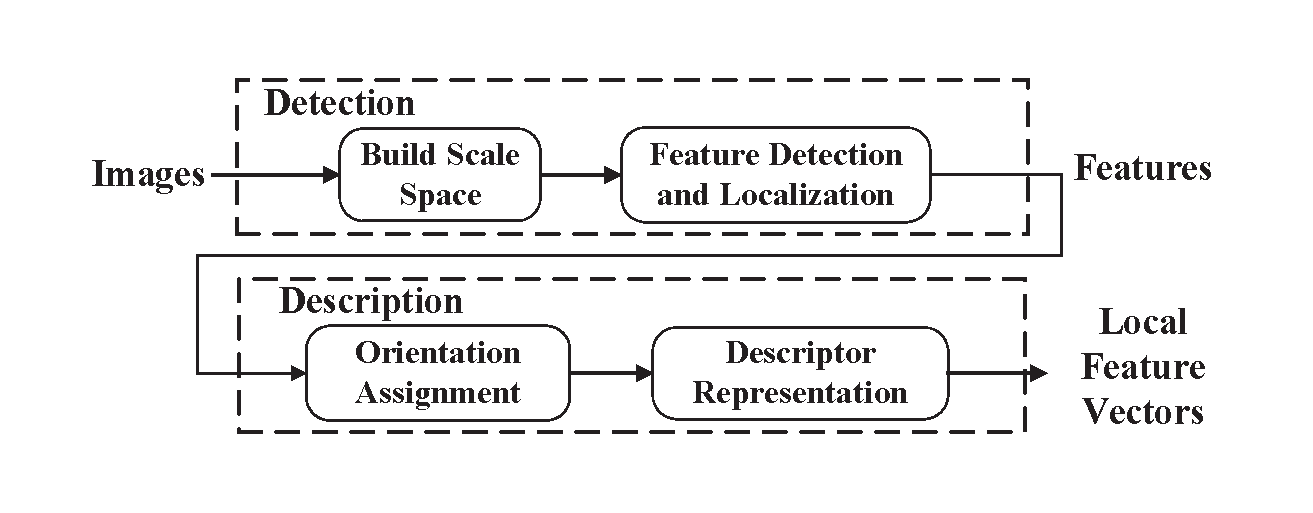
\includegraphics[width=3.8in]{images/fig-workflow.eps}
	\caption{Process flow of a typical local feature descriptor.}
	\label{fig:workflow}
\end{figure}


\begin{figure*}[!ht]
	\centering
	\subfigure[Salient region has the densest local features.]{
		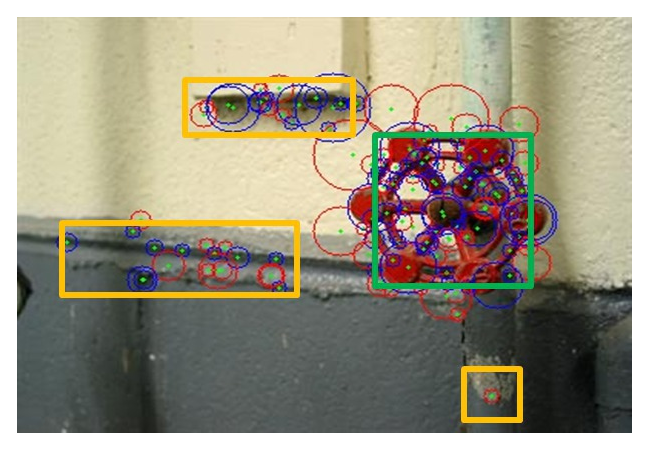
\includegraphics[width=2.2in]{images/fig-observation1.eps}
		\label{fig:observation_1}
	}
	\hfil
	\subfigure[Several salient regions in one image.]{
		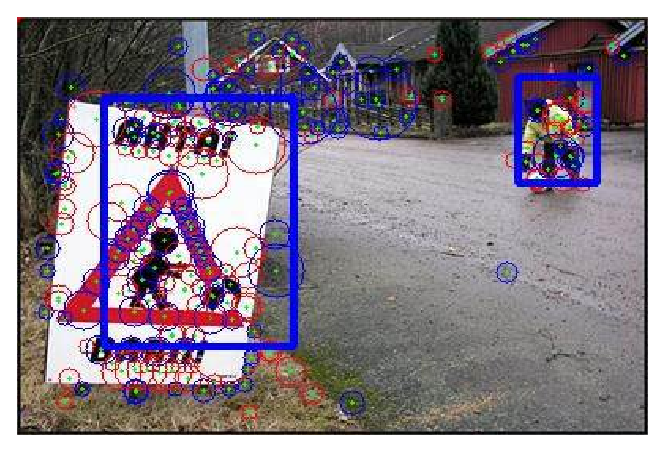
\includegraphics[width=2.2in]{images/fig-observation2.eps}
		\label{fig:observation_2}
	}
	\caption{Example images with local feature based salient regions}
	\label{fig:observations}
\end{figure*}

\squishlist

\item \textbf{Feature Detection:} This stage is to detect \emph{feature points} in an image or a video frame. After an image is initialized, a \emph{m*n} scale space pyramid is constructed to guarantee scale invariant.  After building the scale pyramid, each point in the pyramid is compared with its surrounding 26 points in a 3*3*3 cubic. If its value is the extreme value~(maximum or minimum), the point is chosen as a feature point candidate. To guarantee the quality of extracted points, the candidate points with low contrast or localized along the edges will be discarded. The remaining points are the final feature points.

\item \textbf{Feature Description:} In this stage, each detected point will be described in a high-dimensional vector. First, to make the algorithm rotation invariant, an orientation value is calculated based on the information around it. Then, a descriptor window is constructed and the vector is computed based on the orientation information. The vector value is also normalized to keep the algorithm illumination invariant.
\squishend

There exist two major issues for these {\lfea}s:
\squishlist
\setlength{\itemsep}{0mm}

\item \textbf{Performance issue:} The processing speed of these {\lfea}s are very slow and among their two stages, description stage is more time-consuming as analyzed in \cite{chen2012adaptive}.

\item  \textbf{Storage issue:} {\lfea} usually extract hundreds of feature points to represent an image and use a multi-dimensionality vector~(64 dimension for SURF\cite{bay2006surf} and 128 dimension for SIFT\cite{lowe1999object, lowe2004distinctive}) to represent a feature point, the space requirement is also high to store such a great amount of features.

\squishend

To illustrate these two problems, we evaluate the processing time, the space requirement, the point number and the proportion of execution time between two stages based on the two most widely used algorithms SIFT and SURF which are executed on a i7 Core CPU 4G memory server. The data set was used in ~\cite{mikolajczyk2005performance}. As the data shown in Table \ref{tab:surfandsift}, it can only process less than five images per second and the processing time of description stage is at least twice compared to that of the detection stage. Moreover, there are about one thousand points in each image averagely and each image requires about several hundred KB to storage its feature points.


\begin{table}[!ht]
\begin{center}
\begin{tabular}{|l|c|c|c|c|}
\hline
 & Time(ms) & Space(KB) & Pnum & Proportion \\
\hline
SURF & 171 & 269 & 989   &  1:2\\\hline
SIFT & 719 & 1437 & 2723 & 1:3 \\\hline
\end{tabular}
\end{center}
\caption{Typical time and space consumption of local feature descriptor.}
\label{tab:surfandsift}
\end{table}

As the result shown, for these {\lfea}s, the processing time and the storage space is proportional to the amount of feature points. Less feature points means less processing time and less storage space. In an image or a video frame, there exist some human visual attention regions, called salient regions, these regions are the representative parts in an image or a video frame. If only the feature points in salient regions are extracted, the image can still be represented well and the storage pressure can be released as well. There have been many salient region detection techniques~\cite{cheng2011global,achanta2009frequency,itti1998model}, which picks up visual attention parts from an image. However, prior salient region algorithms cannot satisfy the requirements in terms of processing speed and accuracy. The major constraints come from two aspects:
\squishlist
\item \textbf{Limitation of processing speed:} The goal of a typical salient region algorithm is to detect the visual attention region precisely. Therefore these prior algorithms generally include complex computation, which leads to slow processing speed.

\item \textbf{Limitation of accuracy:} In {\lfea}s, a feature point generally is a extreme point in its local region due to its high contrast. Therefore a lot of local features locate on objects' edges and corners where are also boundaries of salient regions. Since these typical salient region algorithms try to fix the region boundaries precisely, it means the feature points near the boundary cannot be guaranteed to be remained for later retrieval, which would decrease the retrieval accuracy.
\squishend


\subsection{Observation}
\label{subsec:observation}



To overcome these obstacles, we analyze the relation between the salient region and the distribution of feature points in images. We get three major observations:

\begin{description}
	
\item[Observation 1] \desclabel{itm:observation_1} \textit{There exist much denser local features in the salient regions.} It means local features we care about locates close to each other, while noisy features or unimportant features are outside and keep a distance away from them. As shown in Figure \ref{fig:observation_1}, local features in the salient region (green box) gather together and many obviously unimportant points locate far away from that box. Furthermore, our experiment based on 5000 image from~\cite{liu2011learning} show that features points in salient region can be 26 times denser than outside region at most and 3.3 times denser on average.

\item[Observation 2] \desclabel{itm:observation_2} \textit{There may exist several {\sregion}s in an image.} In other words, there exists several clusters of local features in an image. For example, the photo in Figure \ref{fig:observation_2} contains two objects, a person and a stop sign, which shape two {\sregion}s following two clusters of local features.

\item[Observation 3] \desclabel{itm:observation_3} \textit{Local features are close to boundaries of typical salient regions.} From both Figure \ref{fig:observation_1} and Figure \ref{fig:observation_2}, we can observe that most local features locate at objects' edges and corners, which are also the boundaries of typical salient regions.

\end{description}

Observation~\ref{itm:observation_1} indicates that we can detect salient regions directly based on the distribution of local features. In addition, Observation~\ref{itm:observation_2} means it's necessary to deal with the situation of multiple salient regions with multiple clusters of local features in an image. Finally, Observation~\ref{itm:observation_3} shows it's important to avoid eliminating local features on salient regions' boundaries, which require to enlarge actual salient regions to remain these boundary features.


\section{{\sys} Algorithm}
\label{sec:algorithm}

%\subsection{Overview}
%\label{sec:algorithm_overview}

\begin{figure*}[!ht]
\centering
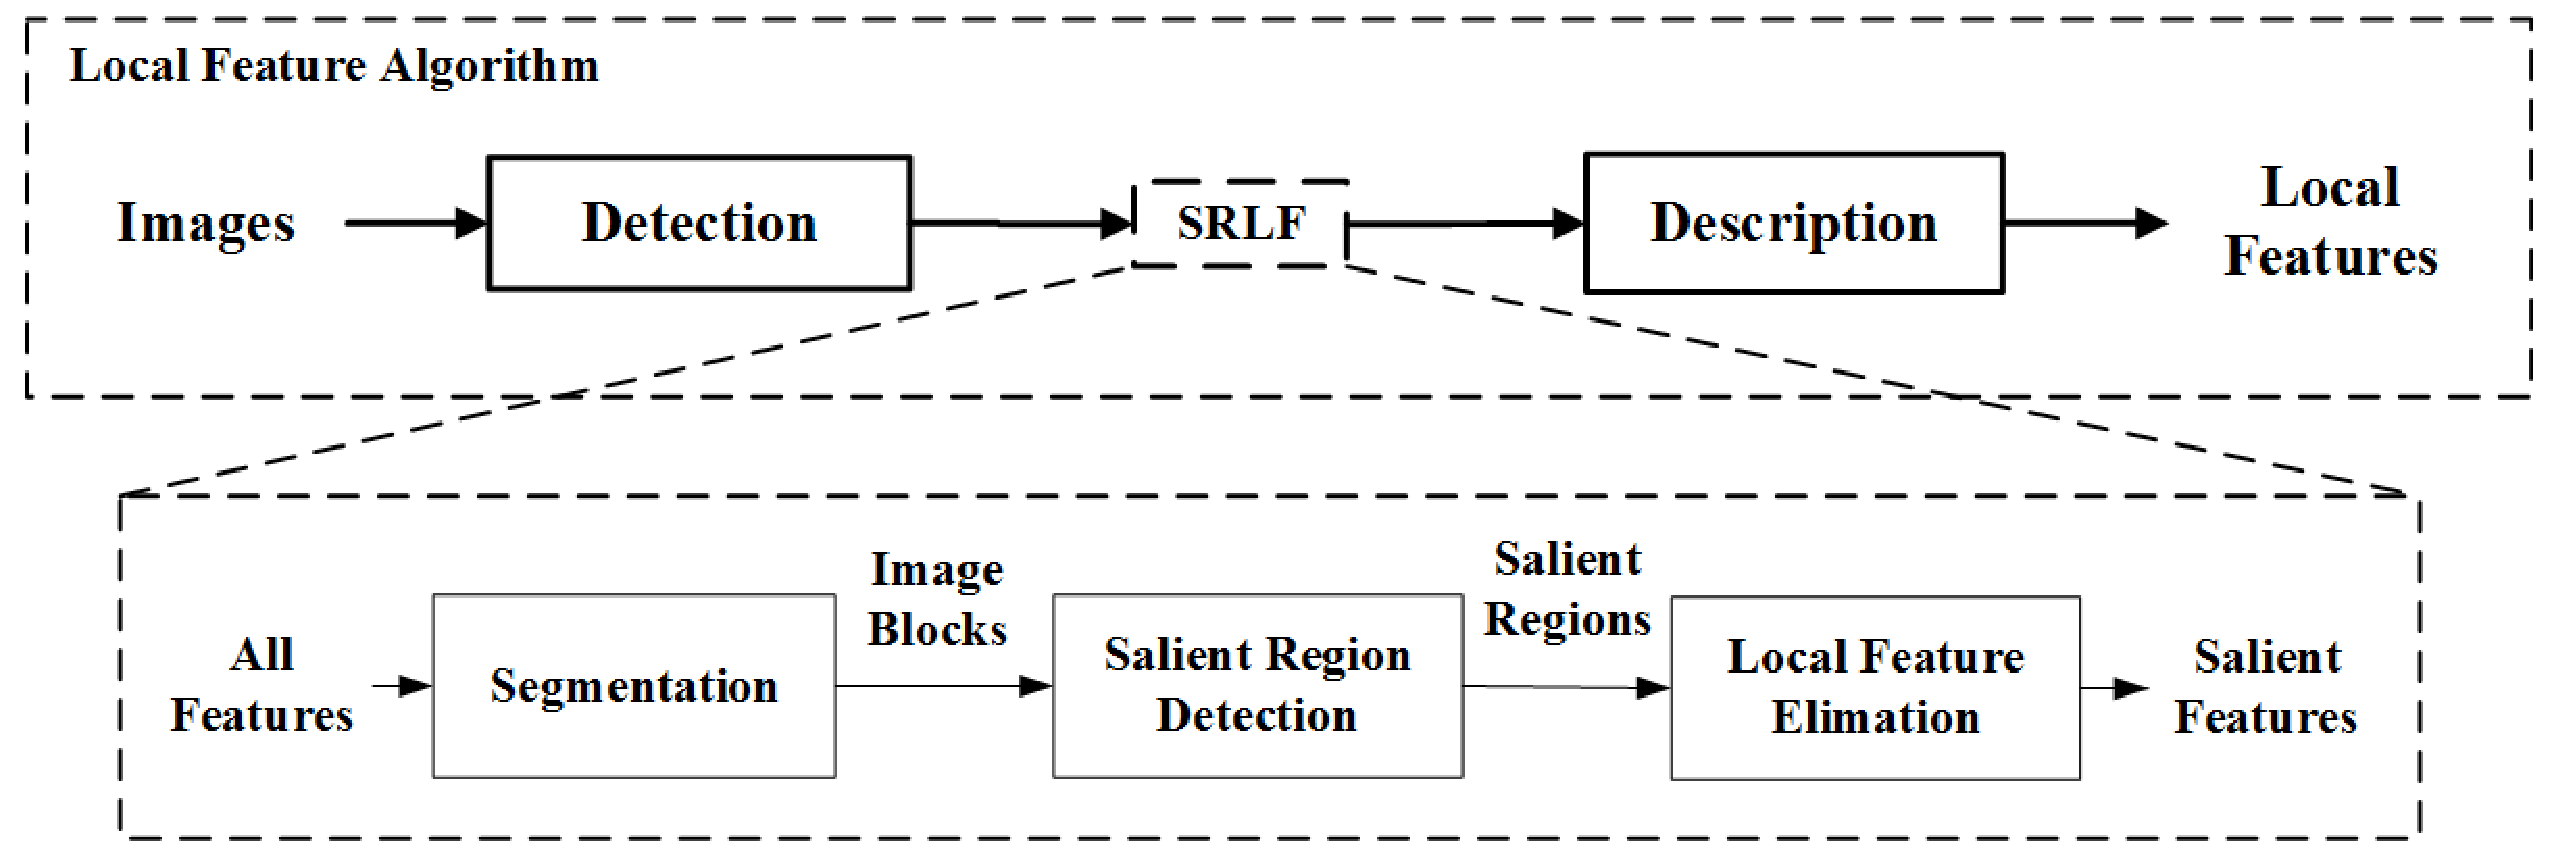
\includegraphics[width=4.5in]{images/fig-overview.eps}
\caption{An overview of {\sys}}
\label{fig:overview}
\end{figure*}

The basic motivation of {\sys} is to design a salient region detection algorithm, which can be used to optimize the obstacles of {\lfea}s and is easy to combined with them. Based on the observations in Section~\ref{subsec:observation}, we design and implement a local feature based salient region algorithm~({\sys}), which is efficient and easy to be combined with {\lfea}s.

As shown in Figure \ref{fig:overview}, {\sys} works as a filter just between the detection stage and the description stage of a typical {\lfea}, where the input of {\sys} is detected feature points and its output is the sets of concerned feature points for computing feature vectors. There exist two major stages in {\sys}.
\begin{itemize}
\item A segmentation step is performed on all local features to identify and partition multiple salient region in an image.
\item For each image segmentation, {\sys} computes that segmentation's salient region individually based on the distribution information of the local feature points in it.
\end{itemize}


\subsection{Local Feature Based Segmentation}
\label{sec:algorithm_segmentation}

According to Observation~\ref{itm:observation_2}, an image may include several salient regions from multiple clusters of local features. Therefore, different clusters need to be identified first. We solve this problem by using a simple segmentation algorithm to divide the image into several blocks based on the distribution of local features. It scans along both the x axis and the y axis from the center of an image. In each scan, a cut-point may be found under the following two constraints:

\begin{itemize}
\item \textit{No local feature could be divided into multiple parts.} In {\lfea}s, scale information is computed to guarantee scale invariant. Therefore, a local feature point is used to represent a region with a radius that equals its scale as shown in Figure~\ref{fig:segmentation}. When the image is partitioned, no segmentation should across the region that a feature point representing.

\item \textit{The cut point should not locate far away from the center.} Each scan is performed from the region center. When the scan goes far, for example 1/4 of the region width, the scan stops and declares that there is no valid cut in that scan. This constraint attends to keep segmentation balanced and avoid too large or too small regions.
\end{itemize}

A typical segmentation is shown in Figure~\ref{fig:segmentation}. The segmentation is started from the center of each axis, e.g. the dot lines in the figure. When a cut-point satisfying the above two constraints is found, the algorithm stops scanning and takes that cut-point as a valid image segmentation, e.g. the solid lines in the figure. After scanning on both the x axis and the y axis, at most four image regions are found in one segmentation.

\begin{figure}[!ht]
\centering
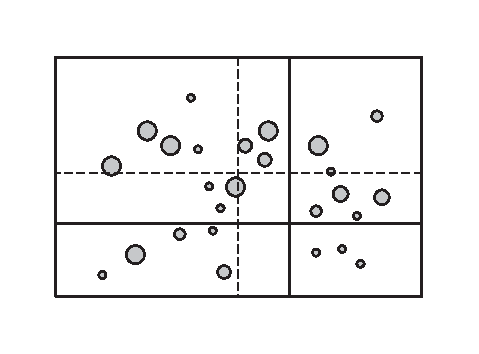
\includegraphics[width=3.3in]{images/fig-segmentation.eps}
\caption{Segmentation by scanning along both the x-axis and y-axis and starting from the dot lines and stops on the solid lines.}
\label{fig:segmentation}
\end{figure}

Then this kind of segmentation will be performed recursively on each image regions. And a recursive segmentation should stop when the following situations are satisfied:

\begin{itemize}
\item \textit{No valid cuts are found.} When no valid cuts following the above two constraints are found, for example a scan exceeds its distance limit, on both x-axis and y-axis of a region, we should regard this region as a whole object and stop performing segmentation on it.

\item \textit{Too few features exist in a region.} Some found regions may have no local feature or just a few features, such as one or two local features, like gray regions in Figure~\ref{fig:segmentation-2}. These regions will be marked as invalid, because they cannot hold one whole object, and no further computation will be performed on them.

\item \textit{The number of segmentations exceeds the limitation.} It's possible that the recursive segmentation becomes too deep if there exist many dispersive points in that region. And actually it makes no sense to perform segmentation on these points, since they cannot be regarded as valid objects individually.

\end{itemize}

\begin{figure}[!ht]
\centering
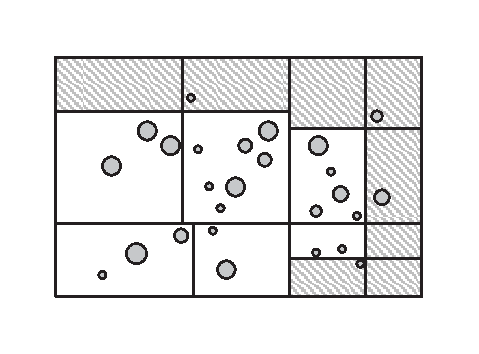
\includegraphics[width=3.3in]{images/fig-segmentation-2.eps}
\caption{Valid and invalid regions after two runs of segmentations. White regions are valid and gray regions are invalid.}
\label{fig:segmentation-2}
\end{figure}


According to our evaluation, in most cases two runs of segmentation are enough, since almost no image has more than sixteen major objects. Thus, it's possible to simplify this processing by performing segmentation only twice in realistic scenarios.

\subsection{Salient Region Detection}
\label{sec:algorithm_detection}

As discussed in Section~\ref{sec:observation}, a precise salient region detection is not suitable for local feature reduction in terms of processing speed and accuracy. Thus, {\sys} employs geometric meaning of local features to compute approximate salient regions.

According to Observation~\ref{itm:observation_1}, the local features in one salient region locate near to each other while noise or unimportant feature points locate far away from them. To simplify this problem, we regard the geometric center of feature points as the center of a salient region. Thus, the region center can be calculated based on the following equation:

{\begin{equation} \label{eq:center}
\left({x}_{c},{y}_{c} \right) = \frac{\sum_{i}^{N}\left({x}_{i},{y}_{i} \right)}{N}
\end{equation}}

Where $\left({x}_{c},{y}_{c} \right)$ means the geometric center of each local feature $\left({x}_{i},{y}_{i} \right)$ in that image segmentation.

After locating the center, we build the final salient regions by expanding the region as a rectangle with a particular width-length ratio. This ratio should be consistent with the distribution of local features, since local features always locate following the shape of target objects. Approximately, this ratio can be considered to equal to the ratio of the dispersion degree on x-axis and y-axis. For example, the bigger dispersion degree of local features on x-axis, the bigger width-length ratio we will get. To compute the ratio of feature dispersions, we can divide the standard deviation of local feature position on x-axis by on y-axis:

{\begin{equation} \label{eq:ratio}
ratio = \sqrt{\frac{\sum_{i}^{N}\left ( x_{i}-x_{c} \right )^{2}}{\sum_{i}^{N}\left ( y_{i}-y_{c} \right )^{2}}}
\end{equation}}

Where $x_{i}$ and $y_{i}$ is a feature's position, while $x_{c}$ and $y_{c}$ is the center position computed by Equation~\ref{eq:center}. To get the final salient region, {\sys} grows the region size until the amount of local feature in it exceeds a desirable number, for example 50 percent of the original local features. As discussed in Observation \ref{itm:observation_3}, this threshold is important for providing a large enough salient region to avoid filtering local features on objects' edges and corners. In our evaluation, we find a ratio about 40\% is proper for most cases.

Combined with segmentation discussed in Section~\ref{sec:algorithm_segmentation}, the processing results will provide several candidate regions. According to Observation \ref{itm:observation_2}, we pick up the candidate regions that have at least 2 local features inside and regard them as the final salient regions.

\subsection{Local Feature Elimination}
\label{sec:algorithm_elimation}

With the knowledge of salient regions in an image, all features locate inside salient regions are kept for further computation, and all other features outside are just dropped. Therefore, we can apply our {\sys} approach to optimize the processing time and the storage requirement. As shown in Figure \ref{fig:overview}, a {\sys}-based local feature extraction algorithm consists of three steps:

\begin{itemize}

\item \textbf{Feature detection:} In this stage, all feature points in an image are detected.

\item \textbf{Salient region detection:} Based on our {\sys} approach, the approximate salient regions in an image are computed based on the distribution of feature points.

\item \textbf{Feature description:} The feature points in the regions are described and the other points are discarded.
\end{itemize}




\section{Evaluation}
\label{sec:evaluation}

In this section, we first give out some comparisons on accuracy. Then show the performance improvement of local feature descriptor by using {\sys}, an evaluation is also performed on {\sys} combined with SIFT and SURF, which are most widely used {\lfea}s. For SIFT, we use an open-source version provided by Rob Hess~\cite{hess2010opensift} as the baseline. For SURF, we also choose an open-source implementation, OpenSURF~\cite{evans2009notes}.

Two data sets are used to satisfy different evaluation purposes.  The first one is a data set of 1000 $640\times480$ images with labeled salient regions by Achanta et at.~\cite{achanta2009frequency}, which is used to evaluate the detection accuracy of salient regions. The second one is a much larger image database provided by Nist~\cite{nister2006scalable}, which consists of 10200 $640\times480$ images for image retrieval system.

The evaluations are performed on a 4-core server with 4GB memory. Each processor is an Intel Core i7 CPU with 3.4Ghz frequency. All the algorithms are compiled by GCC 4.4.0 with optimization argument -O2 under Fedora 11.



\subsection{Experimental Comparison}
\label{sec:evaluation_comparison}

The major motivation of this paper is to design an algorithm for local feature reduction using salient region. To achieve this goal, an approximate salient region detection algorithm is designed. Although our approach cannot detect precise salient region, we are still interested in evaluating its precision against general purpose ones. Here we compare {\sys} with GBSR (Global Contrast based Salient Region)~\cite{cheng2011global}. GBSR is a state-of-the-art salient region detection algorithm, which can achieve the best precision and recall rate compared with prior salient region algorithms. Moreover, it is more efficent than other salient regions detection algorithm. The processing time of GBSR includes two parts: the saliency map detection and its segmentation.

Since we only focus on {\lfea}s, our precision and recall evaluation differs from regular salient region researches a little. As input, we first generate both SURF and SIFT local features for the whole data set. Then we collect the feature points in the salient regions calculated by the ground truth (the regions labelled by Achanta et al. by hand), GBSR and {\sys}. At last, the GBSR's and {\sys}'s precision and recall are calculated based on their results compared with that of the ground truth. In other words, only the local features computed by the ground truth are considered as the truly salient features and the others are false features. Thus, the precision and recall equations are defined as follows.

{\begin{equation} \label{eq:precision}
Precision = \frac{{N}_{correct}}{{n}_{detected}}
\end{equation}}

{\begin{equation} \label{eq:recall}
Recall = \frac{{N}_{correct}}{{N}_{true}}
\end{equation}}

Where ${N}_{correct}$ refers to the number of local features located in both the ground truth and GBSR or {\sys}. ${N}_{detected}$ in equation~\ref{eq:precision} refers to the total number of local features detected by GBSR or {\sys}, while ${N}_{true}$ in equation~\ref{eq:recall} is the number of truly salient features in the ground truth.

\begin{table}[!ht]
\begin{center}
\begin{tabular}{|l|c|c|c|c|c|}
\hline
 & P & R & RE & SM(ms) & SG(ms) \\
\hline
GBSR   & 0.81 & 0.86 & 39\% &180 & 2080 \\
{\sys} & 0.52 & 0.59  & 42\% & N/A & 3 \\
\hline
\end{tabular}
\end{center}
\caption{Comparison between GBSR and {\sys} in precision (P), recall (R), reduction efficiency, saliency map (SM) and segmentation (SG) processing time in milliseconds.}
\label{tab:comparison}
\end{table}

The comparison result is presented in Table~\ref{tab:comparison}. As shown in the column 2 and 3, {\sys} gets lower precision rate and lower recall rate compared to GBSR. The major reason is that our algorithm is an approximate design, which focuses on fast processing speed and accurate retrieval instead of precise boundaries of salient regions. The reduction efficiency in the column 4 refers to the proportion of the left local features after a reduction. The results shows that both of them can help to eliminate more than half of the original features. GBSR achieves a higher reduction rate due to its precise boundary detection.

The result in the column 5 and 6 of Table~\ref{tab:comparison} presents the efficiency comparison, It shows that the well optimized GBSR costs average 2086 milliseconds to get the final salient region for an image, while {\sys} only costs 3.2 milliseconds. Even only counting the time for saliency map detection, GBSR still needs average 178 milliseconds. The performance result of {\sys} is very impressive because the computation of {\sys} is really simple and straightforward.


%-----------------------------------------------------------------------------------------
%-----------------------------------------------------------------------------------------
\subsection{Combination into Retrieval Systems}
\label{sec:evaluation_integration}



{\sys} is designed to improve the performance of {\lfea}s. To verify whether {\sys} satisfies this design purpose, we also evaluate the retrieval accuracy of {\sys} and GBSR. We implement a whole image retrieval system for evaluation. The system first builds a VOC-Tree~\cite{nister2006scalable} by using the feature points extracted by SIFT or SURF from image data sets. Then, each incoming query image is transferred into feature vectors too and retrieved in that VOC-Tree. At last, the found top similar images would be reordered by using RANSAC~\cite{fischler1981random}. In the evaluated data set, four similar images, which are taken from different perspectives for one object, are organized into one group, and for all 10200 images, there are 2550 image groups. When using one image to retrieve, the score of this retrieval is how many images in the same group are found in the top four results. For example, getting three similar images of the query one in the top four retrieval results means a score of 3 and getting nothing similar means a score of 0.

\begin{figure*}[!ht]
\centering
\includegraphics[width=4.5in]{images/fig-gbsr.eps}
\caption{Example feature reduction results conducted by GBSR. From left to right, the first column lists original images, the second column presents binary masks detected by GBSR, and the third column are the local feature reduction result conducted by GBSR, where green points are salient features and red points are filtered ones.}
\label{fig:gbsr}
\end{figure*}

To integrate with salient region algorithm, we replace the original {\lfea} with a salient region conducted version in the image retrieval system. When using an integrated system, the VOC-tree is built based on the feature points in the detected salient regions. Moreover, the retrieval is also based on the feature points in the detected salient regions of a query image.

\begin{table}[!ht]
\begin{center}
\begin{tabular}{|c|c|c|c|}
\hline
\multicolumn{2}{|c|}{} & Query Time & Accuracy \\
\hline
\multirow{3}{*}{SURF} & Original & 0.49s & - \\
& {\sys} &  0.31s & 94\% \\
& GBSR & 2.35s & 93\% \\
\hline
\multirow{3}{*}{SIFT} & Original & 1.5s & - \\
& {\sys} & 0.72s & 93\% \\
& GBSR & 2.58s & 85\% \\
\hline
\end{tabular}
\end{center}
\caption{Comparison between original {\lfea}, {\sys} and GBSR conducted algorithms in a realistic image retrieval system. Query time includes salient region detection and feature detection time, VOC-Tree query time and RANSAC time for the whole image retrieval system. Accuracy refers to the accuracy of the {\sys} and GBSR conducted retrieval system compared to the original ones.}
\label{tab:integration}
\end{table}

Table~\ref{tab:integration} shows the performance results. By reducing local features, the {\sys} conducted image retrieval system gains more than 1.6X speedup for one image query. Although GBSR version has a better reduction efficiency as discussed in the Section~\ref{sec:evaluation_comparison}, the query time becomes worse due to GBSR's long processing time, which leads to longer feature extraction time.

We also present the accuracy influence by introducing {\sys} and GBSR to the retrieval system. In the evaluated data set, four similar images are organized into one group, and for all 10200 images, there are 2550 image groups. For each image retrieval, the score of this retrieval is how many images in the same group are found in the top four results. For example, getting three similar images of the query one in the top four retrieval results means a score of 3 and getting nothing similar means a score of 0.

As shown in the fourth column of Table~\ref{tab:integration}, we get the accuracy by dividing the score of {\sys} and GBSR based algorithms by the score of the original ones. {\sys} based algorithms show a 7\% precision loss. In contrast, GBSR based algorithm shows a more obvious precision loss. When combined with SIFT, the accuracy loss is about 15\%. The major reason behind such a result is that GBSR is a precise silent region detection algorithm. When it used to reduce the feature points in a local feature-based retrieval system, only the points in its detection regions are remained. However, in {\lfea}s, many important points locate in the boundary of an object. To illustrate it clearer, we also give an example shown in Figure~\ref{fig:gbsr}. As the right column shown, many important feature points in the boundary are discarded after GBSR is used, which leads to a larger accuracy loss.


\section{Related Work}

In this section, we first introduce some {\lfea}s. Then we discuss previous salient region detection algorithms and some acceleration efforts on these {\lfea}s.

\subsection{Local Feature-based Algorithms}

There exist many kinds of {\lfea}. SIFT~\cite{lowe1999object, lowe2004distinctive} is the most publicly accepted and robust {\lfea}. For different conditions or purposes, some variants of SIFT are also widely used, such as RIFT~\cite{lazebnik2005sparse}, GLOH~\cite{mikolajczyk2005performance}, and PCA-SIFT~\cite{ke2004pca}. To deal with the performance issue of SIFT, SURF~\cite{bay2006surf} is proposed in 2006 as an optimized local feature descriptor based on SIFT. With acceptable precision loss, SURF tends to be an efficient alternative of SIFT. But the performance of {\lfea}s still far from enormous performance demand as the multimedia data grows shapely. Some researches~\cite{calonder2010brief}\cite{alhwarin2010vf} are trying to improve the feature descriptor structures in order to speed up building and matching features as well as reduce storage.

Local feature descriptors are used widely because of their robustness. Some common applications include automatic image mosaic technique~\cite{yang2008image, salgian2007using}, panorama stitching~\cite{brown2003recognising,tang2008modified}, robot localization~\cite{se2001vision} and object recognition~\cite{heo2008illumination}. And most of them are sensitive to the computation time, or even require real time processing.

\subsection{Salient Region Algorithms}

Most salient region researches focus on generating precise salient map. Some of them~\cite{cheng2011global,achanta2009frequency} have already achieved impressive precision and recall. Inspired by typical salient region algorithm, we try to utilize it to speed up all kinds of {\lfea}s. We are not the first one to take advantage of salient region to improve {\lfea}s. Huang et al.~\cite{huang2009image} involves a salient region detection algorithm to eliminate noises for SURF descriptor. Liang et al.~\cite{liang2010salient} uses similar salient map method to perform noise reduction for SIFT descriptor. But none of them try to improve the computation performance of {\lfea}s by using any salient detection algorithms.

\subsection{Previous Acceleration Efforts}

Since these {\lfea}s include complex computations and have to describe hundreds or even thousands of feature points, they are time-consuming, which limits their application fields with real-time requirements. In order to solve the problem, many efforts have been done to accelerate {\lfea}s through exploiting inherent parallelism in them.

\textbf{Acceleration on Multi-core CPU: }
Zhang et al.~\cite{zhang2008sift} implemented a parallel SIFT algorithm and showed a 6.4X speedup on an 8-core machine. Feng et al.~\cite{feng2008parallelization} achieved a speedup of 11X on a 16-core machine. In~\cite{zhang2009computing}, N. Zhang implemented a scale-level parallelism for SURF on multi-core CPU. In order to overcome imbalanced workload of scale-level, they improved their design with block-level parallelism in~\cite{zhang2010computing}. Although these algorithms can be used to accelerate {\lfea}s, they cannot scale well with the core number increasing. To solve the scalability constraints, Peng et al.\cite{chen2012adaptive} proposed an adaptive pipeline parallelism, which can dynamically adjust the workloads and achieve good scalability.


\textbf{Acceleration on GPGPU: } There are also research of accelerating {\lfea}s on GPGPU, Seth et al.~\cite{warn2009accelerating} explored and evaluated parallel SIFT using large images as input in both multi-core CPU and GPGPU. They found that SIFT requires huge memory space when the input image size is large. Their implementation on a 8-core processor only achieves a speedup of 2X because of the poor cache locality. Their GPGPU version is 13X faster. Sinha et al.~\cite{sinha2011feature} also tried to map SIFT on GPGPU, and their implementation can process 640*480 images at a speed of 10 frames/s on GeForce 7800 GTX. Heymann et al.~\cite{heymann2007sift} presented another GPGPU-based acceleration on SIFT and achieved a speed of 20FPS on QuadroFX 3400. Considering the computing power of GPGPU, their performance is not satisfied. In~\cite{cornelis2008fast}, Cornelis et al. used GPGPU to accelerate SURF based on the combination of scale-level parallelism and block-level parallelism.

Compared to these prior efforts, our approach can further reduce the storage requirements and improve the retrieval time except accelerating feature extraction time. Moreover, our approach is orthogonal to these prior parallel works. In other words, our approach can be parallelized to further improve performance.








\section{Conclusion}
\label{sec:conclusion}

In this paper, we present a Salient Region conducted Local Feature algorithm. Instead of computing directly on local image features, {\sys} takes advantage of an approximate salient region detection approach to perform local feature reduction. According to our evaluation, {\sys} can help to improves the performance of SURF descriptor with a 1.6X speedup and can be combined with all kinds of {\lfea}s . Furthermore, when used in a realistic image retrieval system, our algorithm improve the query performance more than 2 times.


%\section*{Acknowledgement}

\label{sec:acknowledgment}

We thank the anonymous reviewers for their insightful comments. This work was funded by China National Natural Science Foundation under grant numbered 60903015, National 863 Program of China under Grant No. 2012AA010905, Key Project of National 863 Program of China under Grant No. 2009AA012201, Key Project of Major Program of Shanghai Committee of Science and Technology under Grant No. 08dz501600,  Fundamental Research Funds for the Central Universities in China and Shanghai Leading Academic Discipline Project (Project Number: B114).

\bibliographystyle{abbrv}
\bibliography{srlf}

\end{document}